\normalfalse \difficiletrue \tdifficilefalse
\correctiontrue

%\UPSTIidClasse{12} % 11 sup, 12 spé
%\newcommand{\UPSTIidClasse}{12}

\exer{Mouvement RT -- RSG  $\star\star$ \label{C2:08:08}}
\setcounter{question}{0}\UPSTIcompetence[2]{C2-08}
\UPSTIcompetence[2]{C2-09}
\index{Compétence C2-08}
\index{Compétence C2-09}
\index{Torseur cinétique}
\index{Torseur dynamique}
\index{Mécanisme à 1 rotations, 1 translation et RSG}
\ifcorrection
\else
\marginnote{\textbf{Pas de corrigé pour cet exercice.}}
\fi

\ifprof
\else
Soit le mécanisme suivant. On a $\vect{IA}=R\vect{j_0}$ et $\vect{AB}=\lambda(t)\vect{i_1}$. De plus $R=\SI{15}{mm}$.
On fait l'hypothèse de roulement sans glissement au point $I$. De plus :
\begin{itemize}
\item $G_1$ désigne le centre d'inertie de \textbf{1} tel que $\vect{AG_1}=-\ell\vect{i_1}$, on note $m_1$ la masse de \textbf{1} et $\inertie{G_1}{1}=\matinertie{A_1}{B_1}{C_1}{0}{0}{0}{\bas{1}}$; 
\item $G_2=B$ désigne le centre d'inertie de \textbf{2}, on note $m_2$ la masse de \textbf{2} et $\inertie{G_2}{2}=\matinertie{A_2}{B_2}{C_2}{0}{0}{0}{\bas{2}}$.
\end{itemize}
\begin{center}
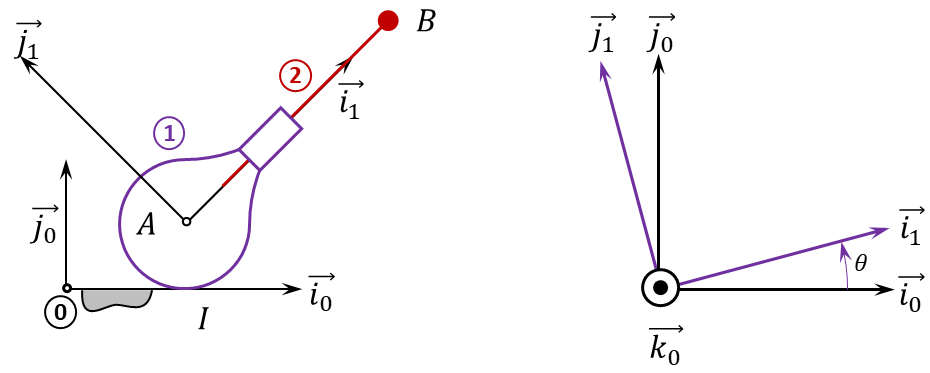
\includegraphics[width=\linewidth]{09_RT_RSG_01}
\end{center}

On donne  $\vectv{B}{2}{0} = \lambdap\vi{1} + \thetap\left(\lambda(t)\vj{1}-R\vi{0} \right)$
et

$\vectg{B}{2}{0}  = \lambdapp(t)\vi{1} %+\lambdap(t)\thetap\vj{1} 
+ \thetapp(t)\left(\lambda(t)\vj{1}-R\vi{0} \right)
+ \thetap(t)\left(2\lambdap(t)\vj{1}-\lambda(t)\thetap\vi{1} \right)
$.


\fi



\question{Déterminer $\vectrd{2}{0}\cdot \vect{i_1}$}
\ifprof

Par définition, $\vectrd{2}{0} =  m_2 \vectg{G_2}{2}{0}=  m_2 \vectg{B}{2}{0}$.

\vspace{.5cm}

\textbf{Calcul de $ \vectv{B}{2}{0}$ :}

$\vectv{B}{2}{0}=\vectv{B}{2}{1}+\vectv{B}{1}{0}$.

D'une part,  $\vectv{B}{2}{1}=\lambdap\vi{1}$.

D'autre part, en utilisant le roulement sans glissement en $I$, 
$\babarv{B}{I}{1}{0} $ $=\vect{0}+\left(-\lambda(t)\vi{1}-R\vj{0} \right)\wedge\thetap \vk{0}$
$=-\thetap\left(\lambda(t)\vi{1}\wedge \vk{0}+R\vj{0}\wedge \vk{0} \right)$
$=\thetap\left(\lambda(t)\vj{1}-R\vi{0} \right)$.

Au final, $\vectv{B}{2}{0} = \lambdap\vi{1} + \thetap\left(\lambda(t)\vj{1}-R\vi{0} \right)$.

\vspace{.5cm}

\textbf{Calcul de $ \vectg{B}{2}{0}$ :}

$\vectg{B}{2}{0} = \deriv{\vectv{B}{2}{0}}{\rep{0}}$
$ = \lambdapp(t)\vi{1} +\lambdap(t)\thetap\vj{1} 
+ \thetapp(t)\left(\lambda(t)\vj{1}-R\vi{0} \right)
+ \thetap(t)\left(\lambdap(t)\vj{1}-\lambda(t)\thetap\vi{1} \right)
$.

Au final, $\vectrd{2}{0} =  m_2 \left( \lambdapp(t)\vi{1} +\lambdap(t)\thetap\vj{1} 
+ \thetapp(t)\left(\lambda(t)\vj{1}-R\vi{0} \right)
+ \thetap(t)\left(\lambdap(t)\vj{1}-\lambda(t)\thetap\vi{1} \right)\right)$
\else
\fi

\question{Déterminer $\vectmd{I}{1+2}{0}\cdot \vect{k_0}$}
\ifprof
On a $\vectmd{I}{1+2}{0} = \vectmd{I}{1}{0} + \vectmd{I}{2}{0}$.

\textbf{Calcul $\vectmd{I}{1}{0}$}

Par déplacement du moment dynamique, on a 
$\vectmd{I}{1}{0} = \vectmd{G_1}{1}{0} + \vect{IG_1}\wedge \vectrd{1}{0}$
\begin{itemize}
\item $\vectmd{G_1}{1}{0}\cdot \vect{k_0} $ $= \deriv{\vectmc{G_1}{1}{0}}{\rep{0}} \cdot \vect{k_0} $ $=C_1 \ddot{\theta}$.
\item $\vectrd{1}{0} = m_1\deriv{\vectv{G_1}{1}{0}}{\rep{0}}$ et  
$\babarv{G_1}{I}{1}{0} $ $=\vect{0}+\left(\ell\vi{1}-R\vj{0} \right)\wedge\thetap \vk{0}$
$=\thetap\left(-\ell\vj{1}+R\vi{0} \right)$. 
On a donc $\vectrd{1}{0} = m_1\thetapp\left(-\ell\vj{1}+R\vi{0} \right)+m_1\ell\thetap^2\vi{1}$.
\item $ \left(\vect{IG_1}\wedge \vectrd{1}{0}\right)  \cdot \vect{k_0}$ 
$ = \left(\left(R\vect{j_0}-\ell\vi{1}\right)\wedge\left( m_1\thetapp\left(-\ell\vj{1}+R\vi{0} \right)+m_1\ell\thetap^2\vi{1}\right)\right)\cdot \vect{k_0}$

$ = \left(R\vect{j_0}\wedge\left( m_1\thetapp\left(-\ell\vj{1}+R\vi{0} \right)+m_1\ell\thetap^2\vi{1}\right)
-\ell\vi{1}\wedge\left( m_1\thetapp\left(-\ell\vj{1}+R\vi{0} \right)+m_1\ell\thetap^2\vi{1}\right)\right)\cdot \vect{k_0}$

$ = m_1\left(R\vect{j_0}\wedge\left( \thetapp\left(-\ell\vj{1}+R\vi{0} \right)+\ell\thetap^2\vi{1}\right)
-\ell \thetapp\vi{1}\wedge\left(-\ell\vj{1}+R\vi{0} \right)\right)\cdot \vect{k_0}$

$ = m_1\left(R\left( \thetapp\left(-\ell\vect{j_0}\wedge\vj{1}+R\vect{j_0}\wedge\vi{0} \right)+\ell\thetap^2\vect{j_0}\wedge\vi{1}\right)
-\ell \thetapp\left(-\ell\vi{1}\wedge\vj{1}+R\vi{1}\wedge\vi{0} \right)\right)\cdot \vect{k_0}$

$ = m_1\left(R\left( \thetapp\left(-\ell\sin\theta-R \right)-\ell\thetap^2\cos\theta\right)
-\ell \thetapp\left(-\ell-R\sin\theta \right)\right)$

$ = m_1\left(-R\left( \thetapp\left(\ell\sin\theta+R \right)+\ell\thetap^2\cos\theta\right)
+\ell \thetapp\left(\ell+R\sin\theta \right)\right)$

$ = m_1\left( -R\thetapp\ell\sin\theta-R^2\thetapp  -R\ell\thetap^2\cos\theta
+\ell^2 \thetapp+R\ell \thetapp\sin\theta \right)$

$ = m_1\left(-R^2\thetapp  -R\ell\thetap^2\cos\theta +\ell^2 \thetapp\right)$

\item Au final, $ \vectmd{I}{1}{0} =C_1 \ddot{\theta} + m_1\left(-R^2\thetapp  -R\ell\thetap^2\cos\theta +\ell^2 \thetapp\right)$.
\end{itemize}



\textbf{Calcul $\vectmd{I}{2}{0}$}

Par déplacement du moment dynamique, on a 
$\vectmd{I}{2}{0} = \vectmd{G_2}{2}{0} + \vect{IG_2}\wedge \vectrd{2}{0}$
\begin{itemize}
\item $\vectmd{G_2}{2}{0}\cdot \vect{k_0} $ $= \deriv{\vectmc{G_2}{2}{0}}{\rep{0}} \cdot \vect{k_0} $ $=C_2 \ddot{\theta}$.
\item $ \left(\vect{IG_2}\wedge \vectrd{2}{0}\right)  \cdot \vect{k_0}$ 
$ = \left(R\vj{0}\wedge  \left(  m_2 \left( \lambdapp(t)\vi{1} +\lambdap(t)\thetap\vj{1} 
+ \thetapp(t)\left(\lambda(t)\vj{1}-R\vi{0} \right)
+ \thetap(t)\left(\lambdap(t)\vj{1}-\lambda(t)\thetap\vi{1} \right)\right)\right)\right)\cdot \vect{k_0}$
$ =  m_2 R \left(\vj{0}\wedge   \left( \lambdapp(t)\vi{1} +\lambdap(t)\thetap\vj{1} 
+ \thetapp(t)\left(\lambda(t)\vj{1}-R\vi{0} \right)
+ \thetap(t)\left(\lambdap(t)\vj{1}-\lambda(t)\thetap\vi{1} \right)\right)\right)\cdot \vect{k_0}$

$ \lambda(t)\vi{1}\wedge  \left(  m_2 \left( \lambdapp(t)\vi{1} +\lambdap(t)\thetap\vj{1} 
+ \thetapp(t)\left(\lambda(t)\vj{1}-R\vi{0} \right)
+ \thetap(t)\left(\lambdap(t)\vj{1}-\lambda(t)\thetap\vi{1} \right)\right)\right)\cdot \vect{k_0}$


$ =  m_2 R \left(  -\lambdapp(t)\cos\theta +\lambdap(t)\thetap\sin\theta 
+ \thetapp(t)\left(-\lambda(t)\sin\theta+R \right)
+ \thetap(t)\left(\lambdap(t)\sin\theta+\lambda(t)\thetap\cos\theta \right)\right)$

$ +\lambda(t)  m_2  \left(  2\lambdap(t)\thetap
+ \thetapp(t)\left(\lambda(t)+R\sin\theta \right)
 \right)$
 
 
 
$ =     
-m_2 R\lambdapp(t)\cos\theta 
+m_2 R\lambdap(t)\thetap\sin\theta 
 -m_2 R\thetapp(t)\lambda(t)\sin\theta
 +m_2 R^2\thetapp(t) 
+ m_2 R\thetap(t)\lambdap(t)\sin\theta
+m_2 R\thetap^2(t)\lambda(t)\cos\theta 
+ 2 \lambda(t)  m_2 \lambdap(t)\thetap
+  \thetapp(t) m_2 \lambda(t)^2
+\thetapp(t)\lambda(t)  m_2 R\sin\theta $


$ =     
-m_2 R\lambdapp(t)\cos\theta 
+m_2 R\lambdap(t)\thetap\sin\theta 
 +m_2 R^2\thetapp(t) 
+ m_2 R\thetap(t)\lambdap(t)\sin\theta
+m_2 R\thetap^2(t)\lambda(t)\cos\theta 
+ 2 m_2  \lambda(t)  \lambdap(t)\thetap
+  m_2  \thetapp(t) \lambda(t)^2
$

Au final, $\vectmd{I}{2}{0} =     
-m_2 R\lambdapp(t)\cos\theta 
+m_2 R\lambdap(t)\thetap\sin\theta 
 +m_2 R^2\thetapp(t) 
+ m_2 R\thetap(t)\lambdap(t)\sin\theta
+m_2 R\thetap^2(t)\lambda(t)\cos\theta 
+ 2 m_2  \lambda(t)  \lambdap(t)\thetap
+  m_2  \thetapp(t) \lambda(t)^2 +C_2\thetapp$
%
%$ = \left(R\vect{j_0}\wedge\left( m_1\thetapp\left(-\ell\vj{1}+R\vi{0} \right)+m_1\ell\thetap^2\vi{1}\right)
%-\ell\vi{1}\wedge\left( m_1\thetapp\left(-\ell\vj{1}+R\vi{0} \right)+m_1\ell\thetap^2\vi{1}\right)\right)\cdot \vect{k_0}$
%
%$ = m_1\left(R\vect{j_0}\wedge\left( \thetapp\left(-\ell\vj{1}+R\vi{0} \right)+\ell\thetap^2\vi{1}\right)
%-\ell \thetapp\vi{1}\wedge\left(-\ell\vj{1}+R\vi{0} \right)\right)\cdot \vect{k_0}$
%
%$ = m_1\left(R\left( \thetapp\left(-\ell\vect{j_0}\wedge\vj{1}+R\vect{j_0}\wedge\vi{0} \right)+\ell\thetap^2\vect{j_0}\wedge\vi{1}\right)
%-\ell \thetapp\left(-\ell\vi{1}\wedge\vj{1}+R\vi{1}\wedge\vi{0} \right)\right)\cdot \vect{k_0}$
%
%$ = m_1\left(R\left( \thetapp\left(-\ell\sin\theta-R \right)-\ell\thetap^2\cos\theta\right)
%-\ell \thetapp\left(-\ell-R\sin\theta \right)\right)$
%
%$ = m_1\left(-R\left( \thetapp\left(\ell\sin\theta+R \right)+\ell\thetap^2\cos\theta\right)
%+\ell \thetapp\left(\ell+R\sin\theta \right)\right)$
%
%\item Au final, $ \vectmd{I}{1}{0} =C_1 \ddot{\theta} +  m_1\left(-R\left( \thetapp\left(\ell\sin\theta+R \right)+\ell\thetap^2\cos\theta\right)
%+\ell \thetapp\left(\ell+R\sin\theta \right)\right)$.
\end{itemize}

\else
\fi


\ifprof
\else
\begin{flushright}
\footnotesize{Corrigé  voir \ref{C2:08:08}.}
\end{flushright}%
\fi